\documentclass[10pt,a4paper]{article}
	
	\usepackage{amsmath,amssymb,amsthm,mathtools,amsfonts}
	\usepackage{breqn}
	\usepackage[utf8]{inputenc}
	\usepackage[english]{babel}
	\usepackage[T1]{fontenc}
	\usepackage{graphicx}
	\graphicspath{{../img/}}
	
	%\usepackage{ebgaramond}
	\usepackage{fontspec}
	\setmainfont[Numbers=OldStyle]{EB Garamond}
	\newfontfamily\mysectionfont[Numbers=OldStyle]{Klavika light}
	
	\usepackage[pdfborder={0 0 0}]{hyperref} %% Ingen firkant rundt om referencer
	\usepackage{multicol}
	\usepackage{tabularx}
	\usepackage{enumitem}% better controls with enumerating
	\usepackage{wrapfig}
		%\setlength{\wrapoverhang}{\marginparwidth}
		%\addtolength{\wrapoverhang}{\marginparsep}
		\setlength{\columnsep}{0pt}
		\setlength{\intextsep}{-10pt}
	\usepackage{caption}
	\usepackage[svgnames]{xcolor}
	\usepackage{dirtytalk}
	\usepackage[modulo]{lineno}
	\usepackage{hyperref}
	\usepackage{pdfpages}
	\usepackage{tasks}
	\newcommand\svar[1]{\newline\textcolor{red}{\textbf{Svar}\\#1}}
	\newcommand{\qm}[1]{“#1”}
	
	\definecolor{hgblue}{RGB}{10, 40, 80}
	\definecolor{hgred}{RGB}{140, 10, 10}
	\definecolor{hggrey}{RGB}{215, 215, 210}
	\definecolor{hggreen}{RGB}{145, 205, 205}
	
	\usepackage{titlesec}
	\titleformat{\subsection}{\color{hgred}\mysectionfont\large}{}{}{}
	\newcommand{\source}[1]{Source: \href{#1}{#1}}
	\usepackage{lipsum}
	\usepackage{comment}
	\usepackage{ulem}
	
	%\reversemarginpar
	\newcommand{\glos}[3]{\dotuline{#1}\marginpar{\scriptsize\textit{#3} #2}}

	\setlength{\parskip}{0.5\baselineskip}
	\setlength{\parindent}{0cm}
	\setlist[enumerate]{label=\alph*),left=20pt}
	%\setlist[enumerate]{leftmargin=\parindent}
	%\setlist[enumerate]{nosep}
	
	%Titling
	\usepackage{titling}
	\setlength{\droptitle}{-12ex}
	\pretitle{\begin{center}\mysectionfont\Huge\color{hgblue}}
	\posttitle{\end{center}}
	\preauthor{\begin{center}\mysectionfont\Large\color{hgblue}}
	\postauthor{\end{center}}
	\predate{\begin{center}\mysectionfont}
	\postdate{\end{center}}
	
	\setcounter{secnumdepth}{0}
	
	\usepackage{tikz}

\begin{document}

%\pagecolor{FloralWhite}
\title{Årsprøve t EN 2021}
%\date{\vspace{-5em}} % I tilfældet ingen dato
\date{Sommer, 2023}
\author{Spørgsmål 16}
\maketitle

\begin{tikzpicture}[remember picture,overlay]
    \node[anchor=north east,yshift=-15pt,xshift=-45pt]%
       at (current page.north east)
        {\includegraphics[scale=0.1]{HG_logo_navn.PNG}};
    \end{tikzpicture}

\thispagestyle{empty}

\vspace{-4em}

\begin{center}
{\color{hgblue}\rule{1\textwidth}{1pt}}
\end{center}

\subsection{Prøvemateriale}
\begin{description}
\item[Theme:] Being American
\item[Text:] Barack Obama, “Democratic National Convention Speech” (2020) (speech) (abridged)
\item[Instruction:] You must analyse and interpret the “Democratic National Convention Speech” by Barack Obama and make a presentation (roughly 8 minutes) of the text and relate it to the theme. Apart from your own points, you must include the following points in your presentation:
\begin{itemize}
\item intention and message
\item use of rhetorical devices
\end{itemize}
\end{description}

\subsection{Bedømmelseskriterier, stx A}
Ved den \textbf{mundtlige prøve} lægges der vægt på, at eksaminanden
\begin{itemize}
\item behersker et flydende og nuanceret engelsk med høj grad af grammatisk korrekthed og evne til
selvkorrektion
\item giver en velstruktureret præsentation
\item analyserer, fortolker og perspektiverer prøvematerialet med anvendelse af fagets analytiske begreber og metoder
\item anvender den viden, der er opnået i arbejdet med det studerede emne.
\item Der lægges i bedømmelsen vægt på, at eksaminanden kan indgå i uddybende samtale om præsentationen.
\end{itemize}
Der gives én karakter ud fra en helhedsvurdering af eksaminandens præstation.
\newpage
\thispagestyle{empty}
\mbox{}

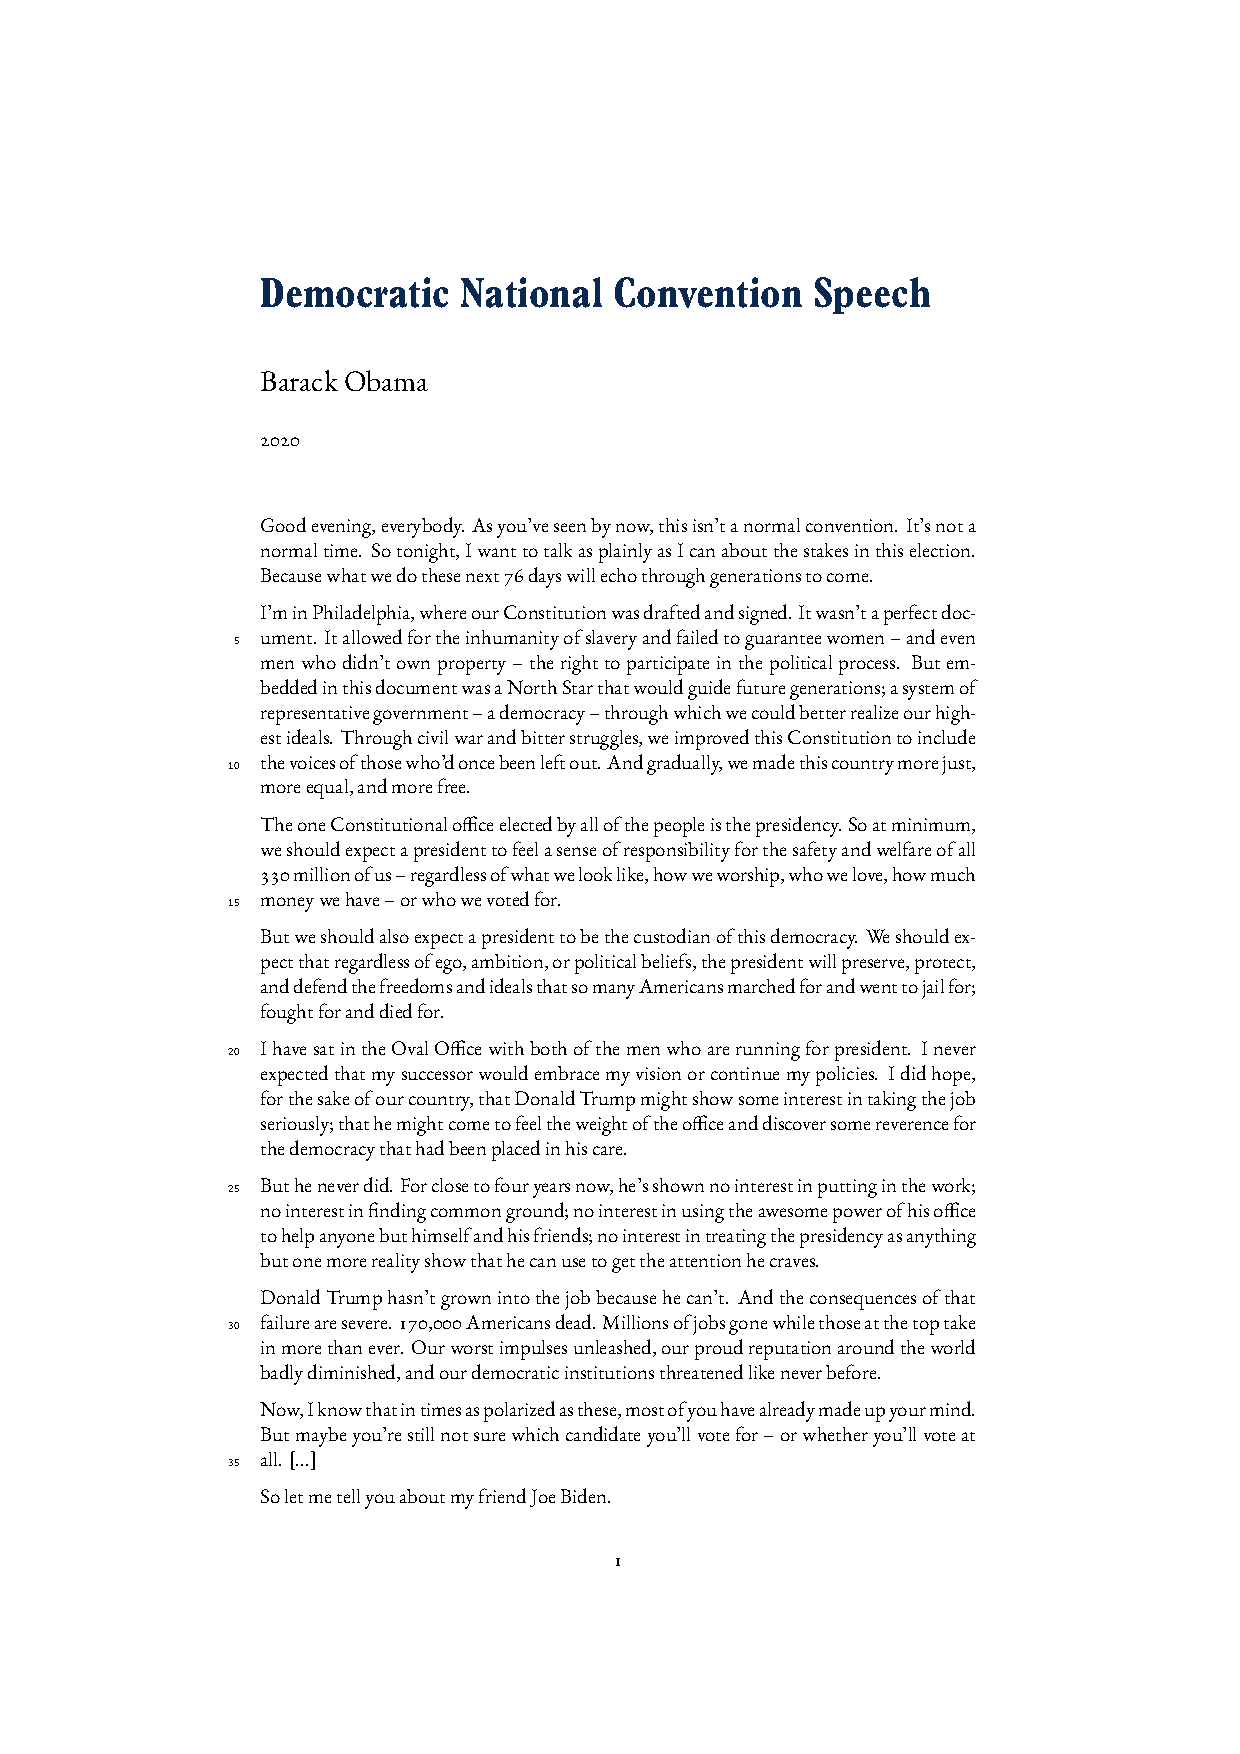
\includepdf[pages=1-]{Obama speech.pdf}






\end{document}


\subsection{Assignment – Short Story (Fiction)}
Write an analytical essay on Haruki Murakami’s short story \qm{On Seeing the 100\% Perfect Girl One Beautiful April Morning}.

Part of your essay must focus on the effect of the short story's preoccupation with dream and reality. It should also include:
\begin{itemize}
\item A \textit{characterisation} of the main character.
\item An intepretation of the short story's \textit{theme} and \textit{message}.
\end{itemize}

Your essay must include references to the short story.


\includepdf[pages=1-]{On Seeing....pdf}